% CS 229 Project Paper
% This is for the milestone; though we're expanding it for the final draft,
% it will probably be useful to have around afterwards.

% Goal: fill three pages with useful background data, plans, stuff.

\documentclass{amsart}
% At this point, my macros file is a bit disorganized. But it ought to be
% usable.

% For page margins
\usepackage[margin=1in]{geometry}
\usepackage{xcolor}
\usepackage{graphicx}
\usepackage{mathtools}
\usepackage{enumerate}
% Sets font to Garamond. Feel free to change this or remove it.
% \usepackage[garamond]{mathdesign}
\usepackage{hyperref}
% Makes figure labels work better
\usepackage[all]{hypcap}

% Note: we might want to use fancyhdr. We can worry about that later.
\pagestyle{plain}

\newcommand{\N}{\mathbb N}
\newcommand{\Z}{\mathbb Z}
\newcommand{\Q}{\mathbb Q}
\newcommand{\R}{\mathbb R}
\newcommand{\T}{^{\mathrm T}\!}
\newcommand{\ud}{\,\mathrm d}
\newcommand{\dfr}[2]{\frac{\mathrm d #1}{\mathrm d #2}}
\newcommand{\pfr}[2]{\frac{\partial #1}{\partial #2}}
\DeclareMathOperator*{\argmax}{arg\,max}
\DeclareMathOperator*{\argmin}{arg\,min}

% I like bold vectors, and this allows bold Greek letters too.
% Feel free to change or remove this.
\renewcommand{\vec}[1]{\boldsymbol{\mathbf{#1}}}

% So that we have \paren{...} instead of \left( and \right)
\DeclarePairedDelimiter\paren{(}{)}
\DeclarePairedDelimiter\ang{\langle}{\rangle}
\DeclarePairedDelimiter\abs{\lvert}{\rvert}
\DeclarePairedDelimiter\norm{\lVert}{\rVert}
% Swap paren* and paren, etc., so that the normal version resizes by default.
% Meanwhile, one can use \paren*[\Big]{...} to customize the size easily.
% It would be interesting to wrap this up into a custom \definedelimiter command...
\makeatletter
    \let\oldparen\paren
    \def\paren{\@ifstar{\oldparen}{\oldparen*}}
    \let\oldang\ang
    \def\ang{\@ifstar{\oldang}{\oldang*}}
    \let\oldabs\abs
    \def\abs{\@ifstar{\oldabs}{\oldabs*}}
    \let\oldnorm\norm
    \def\norm{\@ifstar{\oldnorm}{\oldnorm*}}
\makeatother

% This allows x"i -> x^{(i)} and x"{i+1} -> x^{(i+1)}
\catcode`\"=13
\newcommand{"}[1]{^{(#1)}}

\newcommand{\e}{\varepsilon}
\newcommand{\E}[1]{\cdot 10^{#1}}

\begin{document}
\title{Astronomical Implications of Machine Learning}
\author{
	\lowercase{\href{mailto:adebray@stanford.edu?subject=CS\%20229\%20Project}}{Arun Debray}\\
	\lowercase{\href{mailto:wur911@stanford.edu?subject=CS\%20229\%20Project}}{Raymond Wu}\\
	\today
}
\maketitle

% Do we need a table of contents? Probably not.
%\tableofcontents

% I started writing things. You are welcome to edit them!

% Abstract might not be necessary
\begin{abstract}
In this project we aim to use supervised learning to develop a classifier for stellar lightcurves
 to detect whether they demonstrate the existence of exosolar planets.
\end{abstract}
\section{Introduction}
% What are exoplanets? How are they detected?
The recent discoveries of planets around stars other than our own is among the most significant trends in astronomy today. Long debated by philosophers and physicists alike, no such planets were known until 1992, when two planets were discovered around a star called PSR B1257+12. In the two decades since then, over a thousand such planets have been discovered, diverse in many ways. Thanks to these discoveries, astronomers are learning more about planetary systems other than our own, responding to these questions about other solar systems and even how probable Earth-like life could be in the universe.

In this paper, we will use the following standard terminology.
\begin{itemize}
	\item An \emph{exosolar planet} is defined as in \cite{Ovr} to be a planet that orbits a star other than the Sun.\footnote{The words \emph{exoplanet}, \emph{exosolar planet}, and \emph{extrasolar planet} all mean the same thing, and are used interchangeably.} The standard definition of a planet has two kinds of ambiguity: very low-mass objects in our solar system, such as Pluto, were defined to be ``dwarf planets,'' and the boundaries of this definition aren't entirely clear. Very high-mass planets, however, resemble very small stars; though they don't undergo hydrogen fusion, they look very much like a dim type of star called a brown dwarf. The boundary is somewhat arbitrarily delineated at 13 Jupiter masses. However, neither of these is a great concern in this paper: science is yet unable to detect Pluto-sized worlds around another star, so the low-mass ambiguity does not arise in this data, and the high-mass boundary is not as important: a classifier that discovers planets and small brown dwarfs is still useful. However, it will be helpful to distinguish these systems from eclipsing binaries (see below).
	\item \emph{Planetary transit} is a method of exoplanet detection, In general, because planets are very dim relative to their bright host stars, they cannot be directly imaged, in the same way that it is difficult to detect a firefly near a searchlight from afar. Thus, several indirect methods exist. Planetary transit repeatedly checks the brightness of a star over time; periodic, regular dips in this output sometimes happen because an exoplanet crosses between its sun and the observer. Thus, a planet may be detected without direct observation. See \cite{Trs} for more information on transiting exoplanets.
	\item A \emph{lightcurve} is a graph of a star's brightness over time. A transiting exoplanet will thus manifest itself as a lightcurve that is relatively constant, but with regular, small dips corresponding to the transits. See Figure~\ref{curves} for two examples.
	 The brightness is often given in units of magnitude rather than strict luminosity, because this runs over a relatively nicer range of values.
	\begin{figure}
	\centering
	\label{curves}
	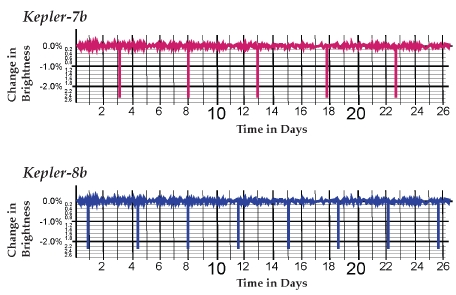
\includegraphics[width=6in]{transit_lightcurve}
	\caption{Lightcurves (graphs of stellar brightness versus time) of two planetary transit systems discovered by Kepler. The regular small dips correspond to the planet passing in front of its sun and slightly diminishing the observed magnitude. Source: NASA}%http://kepler.nasa.gov/education/activities/transitTracks/ if we make a real bibliography
	\end{figure}
	\item An \emph{eclipsing binary} is a pair of stars that orbit each other, but such that each eclipses the other from the Earth's point of view during the orbit. These generally don't contain transiting exoplanets, but instead form an important negative example. Their lightcurves look like those of exoplanets, but they aren't exoplanets.
\end{itemize}
% Why Kepler?

Until recently, most exoplanets weren't detected by transit; astronomers used any of several other methods to find them. However, when the Kepler telescope was launched, it provided a wealth of data about transiting exoplanets, in particular showing that many stars could be surveyed at once. Since Kepler provided such a wealth of data about exoplanets, we decided to try to train a classifier on its lightcurves.%expand? TODO
% Planet Hunters, maybe

\section{Methodology}
We obtained Kepler light curves from the Mikulski Archive for Space Telescopes (see \cite{mast}). Lightcurves are stored in the \texttt{.,fits} file format, so we used the AstroPy Python library, found at \cite{AstroPy}, to process these files. We first divided light curves into those corresponding to exoplanets and those corresponding to non-exoplanets. The light curves are represented as time series data, which means that each light curve is represented by a series of attributes at each time point within some range. The attributes of the light curve stored in the binary table and are data attributes that we are going to be looking at include:
\begin{itemize}
	\item TIME: The time at the midpoint of the light curve
	\item SAP\_FLUX: Simple aperture photometry flux in units of electrons per second contained in the optimal aperture pixels
	\item SAP\_FLUX\_ERR: The error in SAP flux in electrons per second
	\item SAP\_BKG: The total background flux summed over the optimal aperture
	\item SAP\_BKG\_ERR: The error in the background flux
	\item PDCSAP\_FLUX: Flux after Presearch Data Conditioning (PDC) has accounted for systematic error sources such as drift or focus change
	\item PDCSAP\_FLUX\_ERR: The error in PDCSAP flux
	\item PSF\_CENTR1: The column centroid obtained by fitting the point spread function
	\item PSF\_CENTR1\_ERR: The error in PSF centroid 1
	\item PSF\_CENTR2: The row centroid obtained by fitting the point spread function
	\item PSF\_CENTR2\_ERR: The error in PSF centroid 2
	\item MOM\_CENTR1: The column value for the flux weighted centroid (first moment)
	\item MOM\_CENTR1\_ERR: The error in MOM centroid 1
	\item MOM\_CENTR2: The row value for the flux weighted centroid (first moment)
	\item MOM\_CENTR2\_ERR: The error in MOM centroid 2
	\item POS\_CORR1
	\item POS\_CORR2
\end{itemize}

These lightcurves can be thought of as feature vectors in an enormously large-dimensional space, since they correspond to several data points over a large number of distinct observations. Thus, it will be necessary to do some feature selection.

For this milestone, we chose to explicitly work with a few simple features rather than running a larger feature-selection algorithm. Specifically, for each data point above, we calculated the mean and standard deviation of the element over the entire time series. 
%From here we can attempt to do several things. We can try to run some supervised learning classifiers using the arithmetic mean, maximum value, minimum value, range, and standard deviation of each data attribute as opposed to treating it as a time series. 
This primitive form of filtering a time series into its global features is a crude way of using the time series data, but for now it should gives us a rough idea of how our data can be used for classification. We can then use some of the classifiers we learned, such as logistic regression, Na\"ive Bayes classifiers, or support vector machines to train a classifier on these new features. 

We are currently using an optimal margin classifier with the uninteresting

Given that our data is in the form of time series, we will want to look at different forms of time series analysis, such as dynamic time warping or Hidden Markov Models. 

% and so on.
\section{Results}

\section{Analysis}

\section{Future Work}
Since we are dealing with time series data, we want to be able to more powerful tools to see what we can learn more from the data. One possibility is to look at dynamic time warping. Dynamic time warping (DTW), which is an algorithm to measure the similarity between two time sequences that may vary in time or speed. Given that our exoplanets may have varying orbital periods and sizes, DTW may help in detecting more subtle patterns that may be used to distinguish exoplanets or eclipsing binaries. While DTW is a exceptional algorithm, it has one major flaw - it is computionally demanding. Nonetheless, using DTW si definitely another area of improvement we can explore.

% bibliography of some sort
\begin{thebibliography}{9}
\bibitem{AstroPy}{
	Robiatille, Thomas P., et. al.
	\href{http://www.aanda.org/articles/aa/pdf/2013/10/aa22068-13.pdf}{\textit{Astropy: A community Python package for astronomy}}.
	Astronomy and Astrophysics, Volume 558, October 2013.
}
\bibitem{LibLinear}{
	R.-E. Fan, K.-W. Chang, C.-J. Hsieh, X.-R. Wang, and C.-J. Lin.
	\href{http://www.csie.ntu.edu.tw/~cjlin/papers/liblinear.pdf}{\textit{LIBLINEAR: A library for large linear classification}}.
	\href{jmlr.org}{Journal of Machine Learning Research} 9(2008), 1871-1874.
}
\bibitem{Weka}{
	Mark Hall, Eibe Frank, Geoffrey Holmes, Bernhard Pfahringer, Peter Reutemann, Ian H. Witten (2009);
	\href{http://www.sigkdd.org/sites/default/files/issues/11-1-2009-07/p2V11n1.pdf}{\textit{The WEKA Data Mining Software: An Update}};
	SIGKDD Explorations, Volume 11, Issue 1. 
}
% for the general overview, I guess?
\bibitem{Ovr}{
	The Extrasolar Planets Encyclopedia. \url{http://www.exoplanet.eu/} November 15, 2013.
}
\bibitem{Trs}{
	Malatesta, Kerri. \href{http://www.aavso.org/vsots_exoplanets}{\emph{The Transiting Exoplanets HD 209458 and TrES-1}}.
	American Association of Variable Star Observers.
	June 8, 2012.
}
\bibitem{mast}{
	Mikulski Archive for Space Telescopes (MAST).
	\url{http://archive.stsci.edu/kepler/publiclightcurves.html}
	January 30, 2013.
}
\end{thebibliography}
\end{document}
